\documentclass{article}

\usepackage{biblatex}
\addbibresource{../resources.bib}

\usepackage{graphicx}
\usepackage{tikz}
\usetikzlibrary{arrows}
\usetikzlibrary{quantikz}

\usepackage{physics}
\usepackage{amsthm}
\newtheorem{defn}{Definition}
\newtheorem{thm}{Theorem}

\title{Bridging Two-Qubit Gates}
\author{S. S. Kahani}

\def\CNOT{\mathrm{CNOT}}
\def\SWAP{\mathrm{SWAP}}

\begin{document}

In the literature of quantum computing, there is an implementation of $\CNOT$ gate for non-adjacent qubits that share a neighbour, which is called bridge gate~\cite{shende2006,itoko2019}. This implementation is shown in Figure~\ref{fig:3_socalled_bridge}.

% \def\qceq{\midstick[3,brackets=none]{=}}
% \begin{figure}[h]
% \centering
% \begin{quantikz}
%   \lstick{q_1} & \qw &\ctrl{2}&\qw\qceq&\ctrl{1}& \qw    &\ctrl{1}& \qw    & \qw \\
%   \lstick{q_2} & \qw & \qw    & \qw    &\targ{} &\ctrl{1}& \targ{}&\ctrl{1}& \qw \\
%   \lstick{q_3} & \qw &\targ{} & \qw    & \qw    &\targ{} & \qw    & \targ{}& \qw \\
% \end{quantikz}
% \label{fig:3_socalled_bridge}
% \caption{The bridge gate implementation of $\CNOT$ gate.}
% \end{figure}

The importance of such an implementation will be clear when we compare it to the baseline implementation, using the $\SWAP$ gates. The baseline implementation is shown in Figure~\ref{fig:3_baseline_impl}.

\begin{figure}[h]
  \centering
  \begin{quantikz}
  \lstick{q_1} & \ctrl{2} & \qw \qceq & \swap{1} & \qw & \swap{1} & \qw\qceq & \ctrl{1} & \targ{} & \ctrl{1} & \qw &\ctrl{1} & \targ{} & \ctrl{1} & \qw \\
  \lstick{q_2} & \qw & \qw & \swap{} & \ctrl{1} & \swap{} & \qw & \targ{} & \ctrl{-1}& \targ{} & \ctrl{1} & \targ{} & \ctrl{-1}& \targ{} & \qw \\
  \lstick{q_3} & \targ{} & \qw  & \qw & \targ{} & \qw & \qw & \qw & \qw & \qw & \targ & \qw & \qw & \qw & \qw \\
  \end{quantikz}
  \label{fig:3_baseline_impl}
  \caption{The baseline implementation of $\CNOT$ gate.}
\end{figure}

In this paper, we study the possible extenstion the bridge implementation for an arbitrary distance and arbitrary two-qubit gate.

\subsection*{Bridging CNOT gate}

\def\qceq{\midstick[6,brackets=none]{=}}
  \begin{defn}{Generalized Bridge Gate}
    For an even $n$
    \begin{align*} \mathrm{Bridge}(1, n) = &\prod_{i=1}^{n/2 - 1}\mathrm{CNOT}(i + 1, i)\mathrm{CNOT}(n - i + 1, n - i) \\ & \prod_{i=1}^{n/2 - 1}\mathrm{CNOT}(i, i + 1)\mathrm{CNOT}(n - i, n - i + 1) \\ & \mathrm{Bridge}(n/2 - 1, n/2)  \\
    & \qty(\prod_{i=1}^{n/2 - 1}\mathrm{CNOT}(i + 1, i)\mathrm{CNOT}(n - i + 1, n - i))^\dagger \\ 
    & \qty(\prod_{i=1}^{n/2 - 1}\mathrm{CNOT}(i, i + 1)\mathrm{CNOT}(n - i, n - i + 1))^\dagger
    \end{align*}
    but for an odd $n$, it is a little bit different.
  \end{defn}

  \begin{figure}[h]
    \centering
\begin{quantikz}
\qw &\ctrl{5}&\qw\qceq&\targ{}  & \qw     &\ctrl{1}& \qw    & \qw    & \qw    &\ctrl{1}& \qw     &\targ{}&\qw\\
\qw & \qw    & \qw    &\ctrl{-1}&\targ{}  & \targ{}&\ctrl{1}& \qw    &\ctrl{1}&\targ{} &\targ{}  &\ctrl{-1}&\qw\\
\qw & \qw    & \qw    & \qw     &\ctrl{-1}& \qw    & \targ{}&\ctrl{1}&\targ{} & \qw    &\ctrl{-1}&\qw & \qw \\
\qw & \qw    & \qw    & \qw     &\targ{}  & \qw    &\ctrl{1}& \targ{}&\ctrl{1}& \qw    &\targ{}  &\qw & \qw\\
\qw & \qw    & \qw    &\targ{}  &\ctrl{-1}&\ctrl{1}& \targ{}& \qw    &\targ{} &\ctrl{1}&\ctrl{-1}&\targ{}&\qw \\
\qw &\targ{} & \qw    &\ctrl{-1}& \qw     & \targ{}& \qw    & \qw    & \qw    &\targ{} & \qw     &\ctrl{-1}& \qw 
\end{quantikz}
\caption{The bridge gate for $n=6$}
\end{figure}


  As far as we know, the family of bridge gates with more than one qubit in the chain is not studied yet, and neither implemented in any quantum compiler. 
  It can be easily shown that for a simple case like the one in the figure \ref{fig:bridge-simplification} that we need to swap and return the qubits, using bridge gate can reduce both depth and number of gates. 

  \begin{figure}[h]
    a) \\
    \begin{center}
    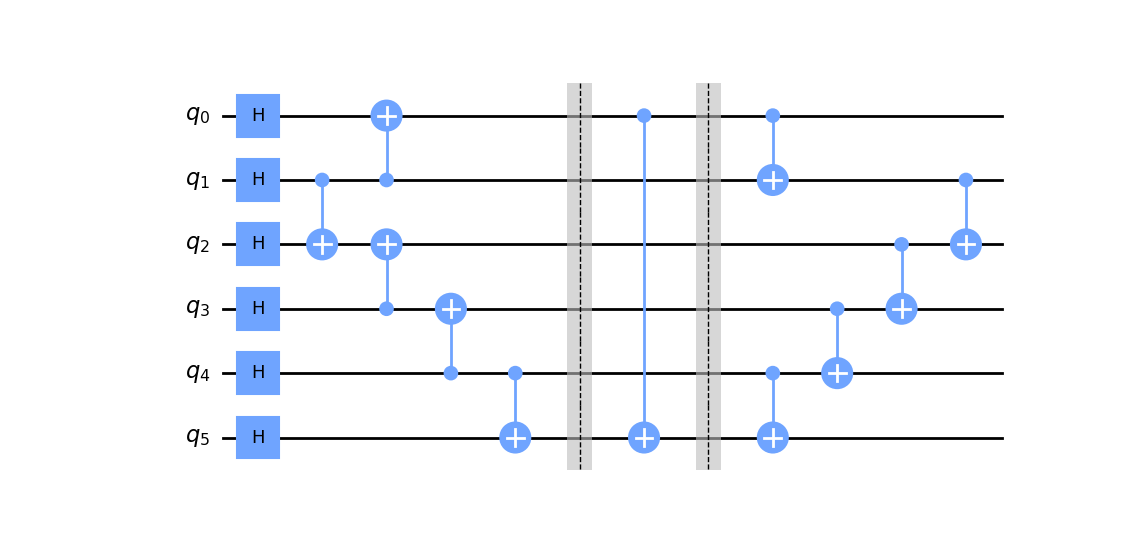
\includegraphics[width=0.9\textwidth]{../../code/expm_1_bridge/out/original_circuit}
    \end{center}
    b) \\
    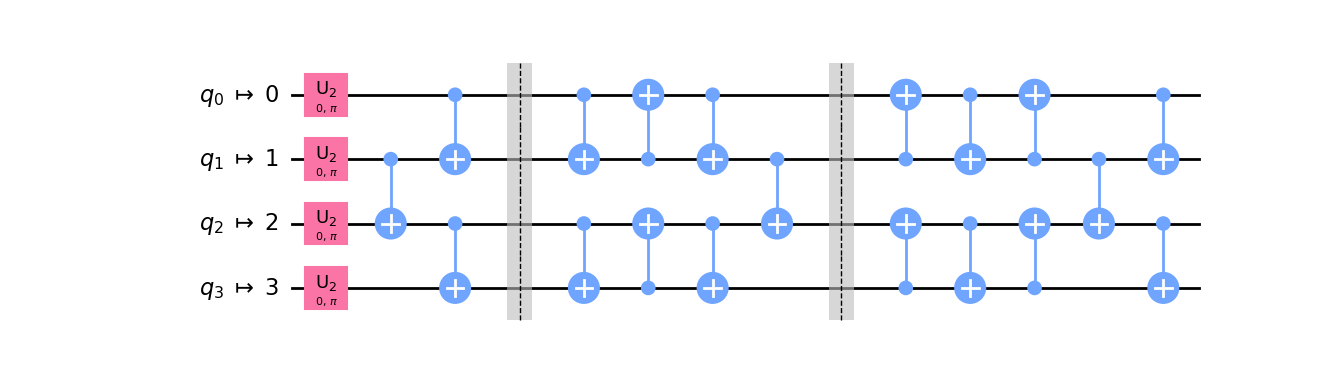
\includegraphics[width=0.9\textwidth]{../../code/expm_1_bridge/out/transpiled_circuit_swap} \\
    c) \\
    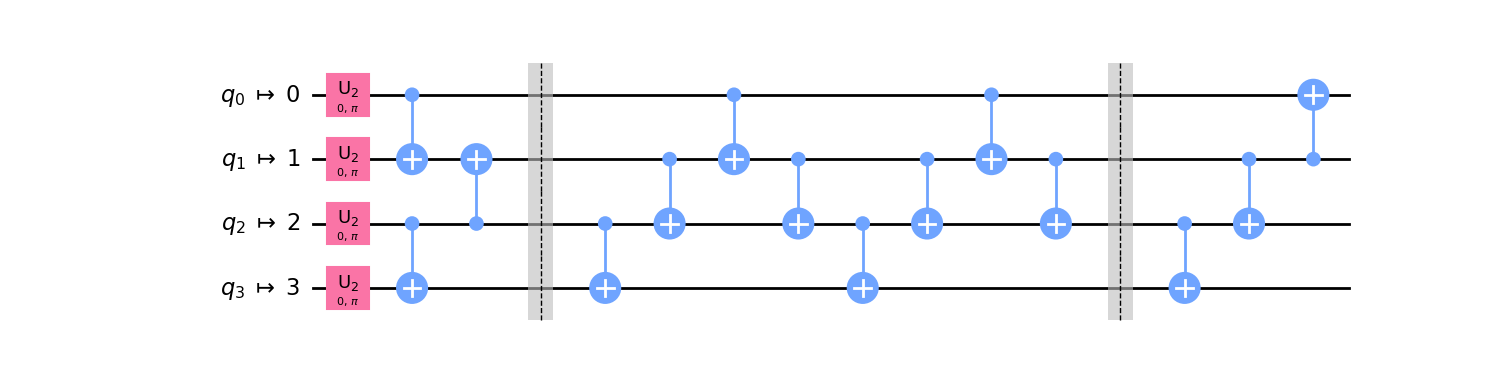
\includegraphics[width=0.9\textwidth]{../../code/expm_1_bridge/out/transpiled_circuit_bridge}
    \caption{a) The original circuit, consisting of some local operations, then a far away CNOT and then some local operations. b) The circuit after transpiling using Qiskit. c) The circuit after transpiling using bridge gate as an intermediate gate.}
  \end{figure}

    Later we prove that this circuit is optimal.

\subsection*{Bridging SWAP gate}

\subsection*{Bridging arbitrary gates}

For any two-qubit gate $U$, we can define $R_\leftarrow$ and $R_\rightarrow$ as the amount of information that can be commuicated back and forth. Note that they may vary for different scenarios of using $U$, (e.g. different initialization).

We know that

\begin{equation}
  \begin{cases} 
    R_{\leftarrow} + R_{\rightarrow} \le E_U \\
    R_{\leftarrow} \le 1 \\
    R_{\rightarrow} \le 1
  \end{cases}
\end{equation}

In case of 


\end{document}


https://ucl.zoom.us/j/98762501915?pwd=WEdPVmFqSW5EZ00wSktrc3BQY290Zz09